\section{Document-Driven Web Development Process}
\label{sec:document-driven web_development_process}

The process to build a web application based on x-learning toolkit consists of the following four steps: models schemas definition, HTTP RESTful API definition, UI components definition and UI components  assembly.


\begin{figure}[htb] %  figure placement: here, top, bottom
 \centering
 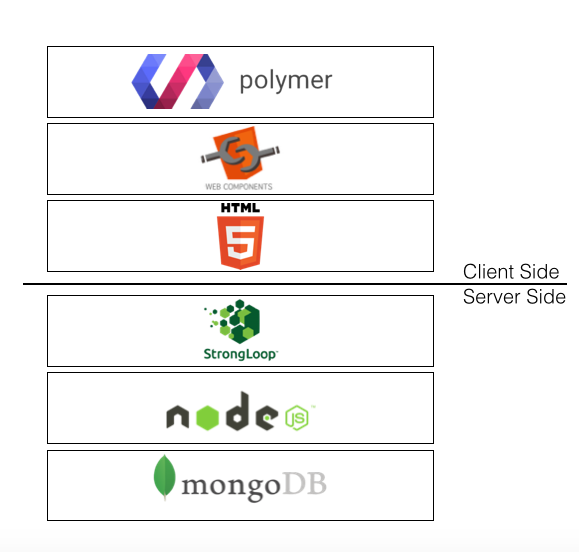
\includegraphics[width=1.0\linewidth]{images/chapter3/XPR_stack.png}\hfill
 \caption[X-learning Architectural Stack]{X-Learning Architectural Stack}
 \label{fig:fourV}
\end{figure}

\subsubsection {1st step - Models schemas definition}
\label{subsec:1st_step_models_schemas_definitio}


A description of entities, properties, relations and data access policies are defined as JSON  documents.
As to a learning platform, the essential entities to be modelled are the following: Course, Lecture, Video and Teacher(Member).

\subsubsection{ Model - Member}

The model Member represents the course creator but also the students of other course. Its features are: name, lastname, email.gender,photo,phone number,location and date. The Member has relations with course, and for each of these relation can be learning or teaching.

\begin{lstlisting}[language=json]
{
  "name": "Member",
  "base": "User",
  "properties": {
    "name": {
      "type": "String"
    },
    "last_name": {
      "type": "String"
    },   
    "birthday": {
      "type": "Date"
    },
    "email": {
      "type": "String"
    },
    "gender": {
      "type": "String"
    },
    "password": {
      "type": "String"
    },
    "photo": {
      "type": "String"
    },
    "location": {
      "type": "String"
    },
    "phone": {
      "type": "Number"
    }
  },
  "relations": {
    "learning": {
      "type": "hasAndBelongsToMany",
      "model": "Course",
      "through": "MemberCourse"
    },
    "teaching": {
      "type": "hasMany",
      "model": "Course",
      "foreignKey": "teacher_id"
    }
  }
}
\end{lstlisting}


\subsubsection{ Model - Course}

The model Course defines the main element structure that must be published. Main features are: title, cost, documentation, publish and publication date. This model has relations with teacher, students, category, lectures and webinars models.


\begin{lstlisting}[language=json]
{
  "name": "Course",
   "properties": {
    "title": {
      "type": "String"
    },
    "description": {
      "type": "String"
    },
    "date": {
      "type": "Date"
    },
    "cover": {
      "type": "String"
    },
    "language": {
      "type": "String"
    },
    "cost": {
      "type": "Number"
    },
    "publish": {
      "type": "Boolean"
    },
    "documents": {
      "type": "Array"
    },
    "skill": {
      "type": "Array"
    }
  },
  "relations": {
    "category": {
      "type": "belongsTo",
      "model": "Category",
      "foreignKey": "category_id"
    },
    "teacher": {
      "type": "belongsTo",
      "model": "Member",
      "foreignKey": "teacher_id"
    },
    "lectures": {
      "type": "hasMany",
      "model": "Lecture",
      "foreignKey": "course_id"
    },
    "webinars": {
      "type": "hasMany",
      "model": "Webinar",
      "foreignKey": "webinar_id"
    },
    "students": {
      "type": "hasAndBelongsToMany",
      "model": "Member",
      "through": "MemberCourse"
    }

\end{lstlisting}

\subsubsection{ Model - Lecture}

The model Lecture defines the single lecture into a determinate course. Main features are: title, description. This model has relations with course, video.


\begin{lstlisting}[language=json]
{
  "name": "Lecture",
  "properties": {
    "title": {
      "type": "String"
    },
    "description": {
      "type": "String"
    }
  },
  "relations": {
    "course": {
      "type": "belongsTo",
      "model": "Course",
      "foreignKey": "course_id"
    },
    "video": {
      "type": "hasOne",
      "model": "Video",
      "foreignKey": "lecture_video_id"
    }
  }

\end{lstlisting}

\subsubsection{ Model - Video}

The model Video defines the video object belong to lecture. Main features are: title, url and duration of its. This model has relations with lecture.


\begin{lstlisting}[language=json]
{
  "name": "Video",
  "properties": {
    "title": {
      "type": "String"
    }
    "url": {
      "type": "String"
    },
    "duration": {
      "type": "Number"
    }
  },
  "relations": {
    "lecture": {
      "type": "belongsTo",
      "model": "Lecture",
      "foreignKey": "lecture_video_id"
    }
  }
}

\end{lstlisting}


\subsubsection {2nd step - HTTP RESTful API definition}
\label{subsec:2nd_step_HTTP_RESTful_API_definition}

CRUD operations on models are automatically generated by the web framework (on the basis of input JSON documents) and further custom actions can be defined. All of them are exposed as HTTP RESTful API.
These models result in the following HTTP RESTful API, automatically generated by Loopback server.

\subsubsection{ Members API}
\begin{itemize}
\item \textbf{GET /api/Members} Find all instances of the model matched by filter from  the  data source.
\item \textbf{POST /api/Members} Update an existing model instance or insert a new one into the data  source.
\item \textbf{PUT /api/Members} Create a new instance of the model and persist it into the data source.
\item \textbf{DELETE /api/Members/id} Delete a model instance by id from the data source.
\item \textbf{GET / Members/id/teaching} {\color{red}Queries teacher course of model.}

\item \textbf{GET / Members/id/learning} {\color{red} Queries follow course of model.}

\item \textbf{POST /api/changeEmail} Change email of a model instance.
\item \textbf{POST /api/changePassword} Change password of a model instance.
\item \textbf{GET /api/count Count} instances of the model matched by where from the  data source.
\item \textbf{POST /api/login} Login a user with username/email and password.
\item \textbf{POST /api/logout} Logout a user with access   token.
\item \textbf{POST /api/reset} Reset password for a user with email.
\item \textbf{POST /api/update} Update instances of the model matched by where from the data source.
\end{itemize}

\subsubsection{ Course API}
\begin{itemize}
\item \textbf{PUT /Courses} Update an existing model instance or insert a new one into the data  source.
\item \textbf{GET /Courses} Find all instances of the model matched by filter from the data  source.
\item \textbf{POST / Courses} create a new instance and persist it into the data source.
\item \textbf{GET / Courses/id/lectures} Queries lectures of course.
\item \textbf{POST / Courses/id/lectures} Creates a new instance in lectures of  this model.
\item \textbf{DELETE / Courses/id/lectures} Deletes all lectures of this model.

\item \textbf{GET / Courses/id/webinars} Queries webinars of course.
\item \textbf{POST / Courses/id/webinars} Creates a new instance in webinars of  this model.
\item \textbf{DELETE / Courses/id/webinars} Deletes all webinars of this model.

\item \textbf{GET / Courses/id/students} Queries students of course.
\item \textbf{POST / Courses/id/students} Creates a new instance in students of  this model.
\item \textbf{DELETE / Courses/id/students} Deletes all students of this model.
\end{itemize}


\subsubsection{ Lectures API}
\begin{itemize}
\item \textbf{GET /api/Lectures} Find all instances of the model matched by filter from  the  data source.
\item \textbf{POST /api/Lectures} Update an existing model instance or insert a new one into the data  source.
\item \textbf{PUT /api/Lectures} Create a new instance of the model and persist it into the data   source.
\item \textbf{DELETE /api/Lectures/id} Delete a model instance by id from the data source.
\item \textbf{GET /api/Lectures/id/course} Fetches belongsTO relation course.

\item \textbf{GET /api/Lectures/id/video} Fetches belongsTO relation video.
\item \textbf{GET /api/Lectures/count} Count instances of the model matched by where from the data  source.
\end{itemize}

\subsubsection{ Images API}

\begin{itemize}
\item \textbf{POST /Model}
\item \textbf{POST /Images} create a new instance and persist it into the data source.
\item \textbf{PUT /Images} Update an existing model instance or insert a new one into the data source.
\item \textbf{GET /Images} Find all instances of the model matched by filter from the  data source.
\item \textbf{POST /Images/upload} Upload a new instance into data source.
\item \textbf{GET /Images/id} Find a model instance by id from the data source
\item \textbf{PUT /Images/id} Update attributes of a model instance and persist it into the data source.
\item \textbf{DELETE /Images/id} Deletes a model instance by id from the data 
source.
\end{itemize}

\subsubsection{ Videos API}
\begin{itemize}
\item \textbf{POST /Videos} create a new instance and persist it into the data source.
\item \textbf{PUT /Videos} Update an existing model instance or insert a new one into the data source.
\item \textbf{GET /Videos} Find all instances of the model matched by filter from the  data source.
\item \textbf{GET /Videos/id} Find a model instance by id from the data source
\item \textbf{PUT /Videos/id} Update attributes of a model instance and persist it into the data source.
\item \textbf{DELETE /Videos/id} Deletes a model instance by id from the data 
source. 
\item \textbf{GET /Videos/id/lecture} Fetches belongsTO relation lecture.
\end{itemize}

\subsubsection{Webinars API}
\begin{itemize}
\item \textbf{POST /Webinars} create a new instance and persist it into the data source.
\item \textbf{PUT /Webinars} Update an existing model instance or insert a new one into the data source.
\item \textbf{GET /Webinars} Find all instances of the model matched by filter from the  data source.
\item \textbf{POST /Webinars/course} Fetches belongsTO relation course.
\item \textbf{GET /Webinars/id} Find a model instance by id from the data source
\item \textbf{PUT /Webinars/id} Update attributes of a model instance and persist it into the data source.
\item \textbf{DELETE /Webinars/id} Deletes a model instance by id from the data 
source.
\end{itemize}

 \subsubsection{ Remote Methods }
  
  Come abbiamo detto per ogni modello vengono generate automaticamente le api dal server di Strongloop. Ogni modello rappresentato da un file JSON è anche accompagnato da un file js che di default si presenta in questo modo definito come hook
  \begin{lstlisting}[language=javascript]

    module.exports = function (x-model) {
    
    };
  \end{lstlisting}


Use model hooks to add custom logic to models that extend PersistedModel. Each hook is called before or after a specific event in the model's lifecycle.
Best practice is to register model hooks in /common/models/x-model.js
Di seguito sono riportate alcuni metodi remoti che sono stati creati e un esempio esplicativo.

\begin{itemize}
\item \textbf{GET /videos/signed\_upload\_part }
\item \textbf{GET /videos/create\_multiPart\_upload}
\item \textbf{PUT /videos/complete\_upload\_part }
\item \textbf{DELETE /videos/delete\_video}
\end{itemize}

\begin{lstlisting}[language=javascript]

module.exports = function (Video) {
  ...
Video.delete_video = function(path,callback) {
    var self = this;
    var params = {
      Bucket: S3_BUCKET,
      Prefix: path
    };

    s3.listObjects(params, function(err, data) {
      if (err){
        console.log(err);
        callback(err);
        return;
      } 

      params = {Bucket: S3_BUCKET};
      params.Delete = {};
      params.Delete.Objects = [];

      data.Contents.forEach(function(content) {
        params.Delete.Objects.push({Key: content.Key});
      });

      s3.deleteObjects(params, function (err, delete_response) {
        if (err){
          console.log(err);
          callback(err);
          return;
        }

        console.log(delete_response.Deleted.length);
        callback(null, delete_response);
      });
    });
  };

  Video.remoteMethod('delete_video', {
    http: { verb: 'delete' },
    accepts: [
      {arg: 'path', type: 'string'}
    ],
    returns: {arg: 'delete_response', type: 'string'}
  });
  ....
};
\end{lstlisting}

\subsubsection {3rd step - UI components definition}
\label{subsec:3rd_step_UI_components_definition}

Distinct UI components can be defined, or retrieved from a collection of predefined components, configured and adapted. They represent the building blocks of the whole UI.
{\color{red}The following is an example:}

\begin{lstlisting}[language=html]
<part-course-actions course="{{course}}"></part-course-actions>
\end{lstlisting}

\begin{figure}[htb] %  figure placement: here, top, bottom
 \centering
 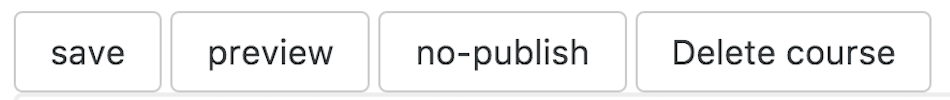
\includegraphics[width=1.0\linewidth]{images/chapter3/admin-course-actions.png}\hfill
 \caption[Page Admin course action]{Page Admin course action}
 \label{fig:fourV}
\end{figure}

\begin{lstlisting}[language=html]
<part-course-info course="{{course}}" error="{{error}}"></part-course-info>
\end{lstlisting}


\begin{figure}[htb] %  figure placement: here, top, bottom
 \centering
 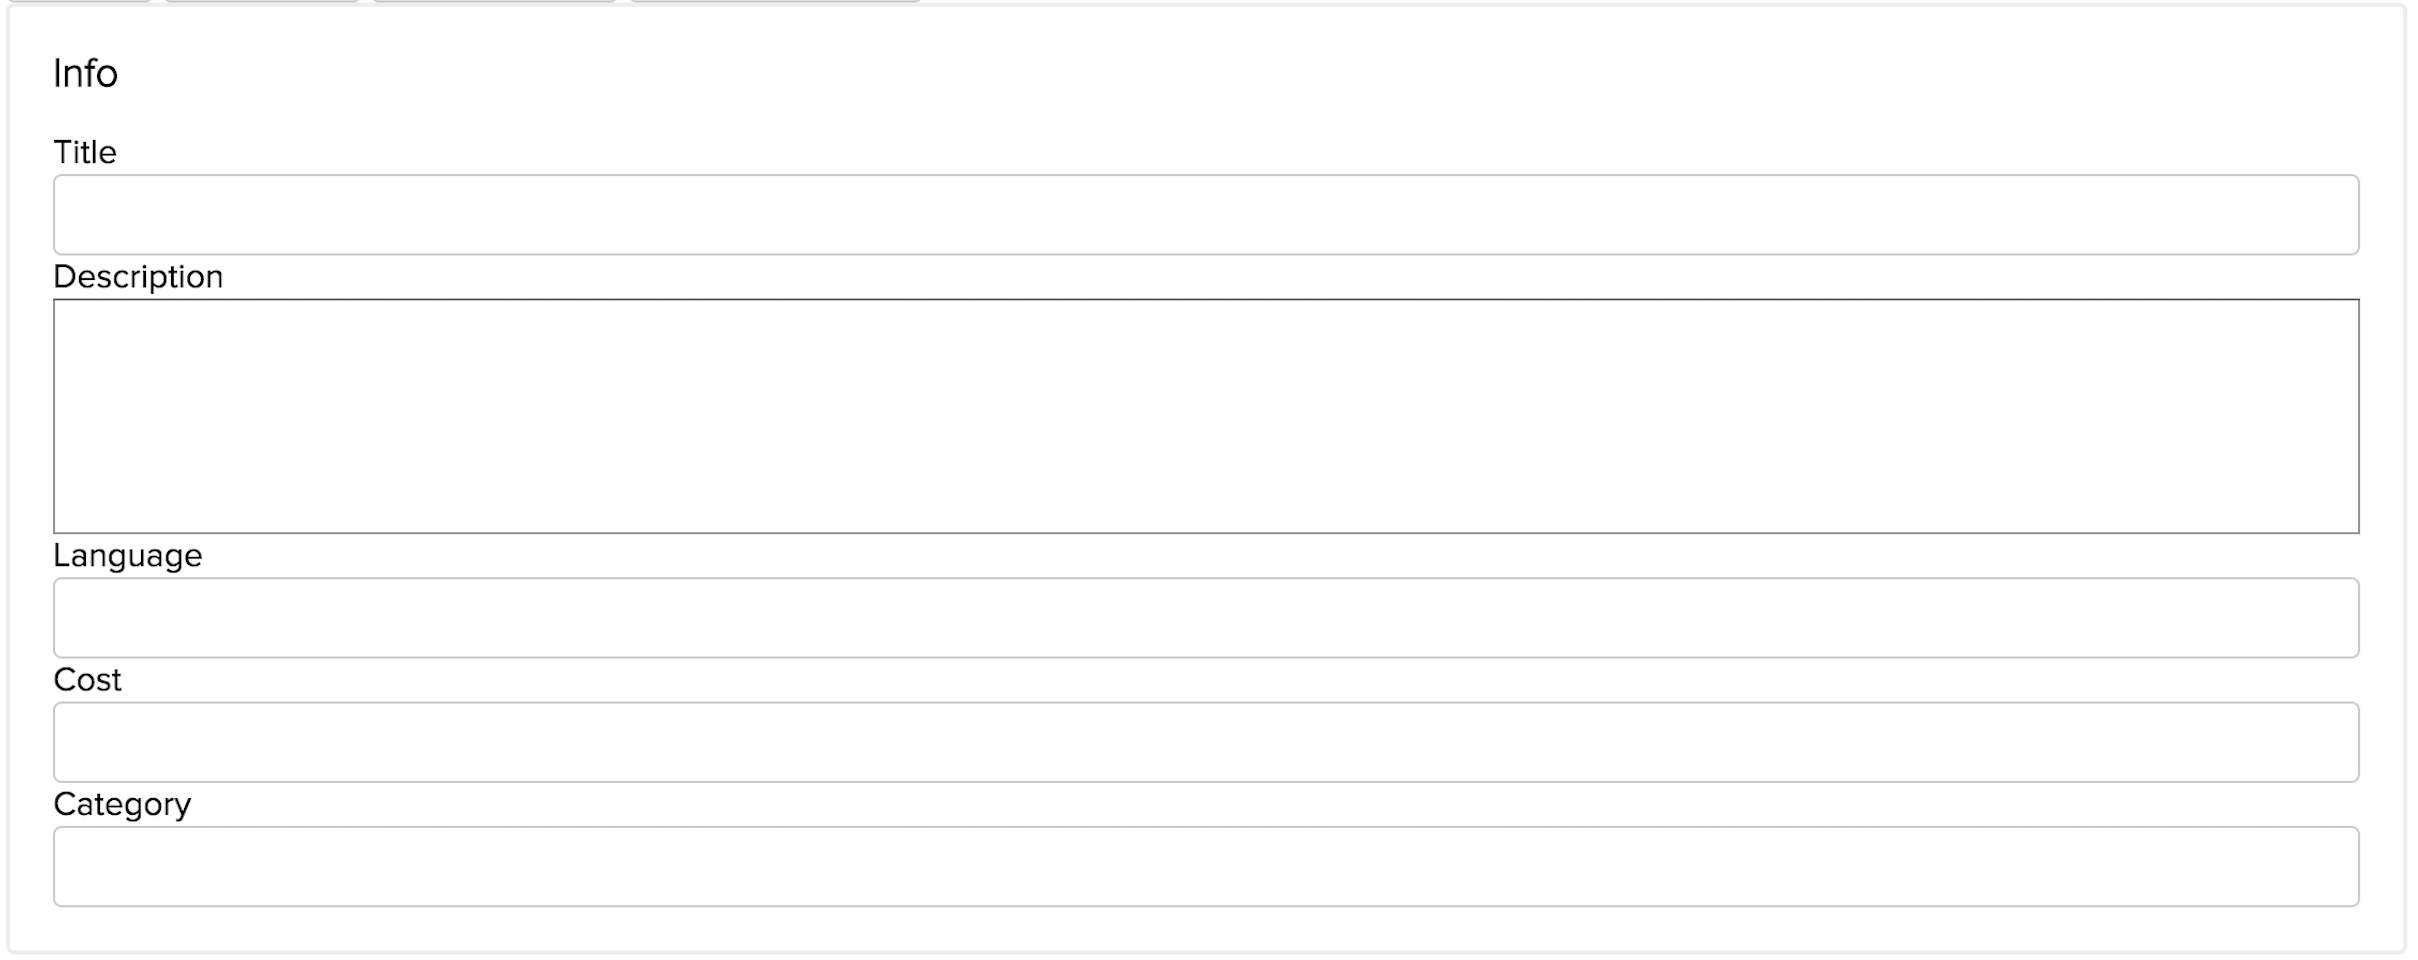
\includegraphics[width=1.0\linewidth]{images/chapter3/admin-course-info.png}\hfill
 \caption[Page Admin course info]{Page Admin course info}
 \label{fig:fourV}
\end{figure}

\subsubsection {4th step - UI components assembly}
\label{subsec:4th_step_UI_components_assembly}

Distinct UI components are finally mounted to compose the application views. Assembly is kept as simple as possible: it only consists of a composition of HTML5 elements. So, the entire development process results driven by: JSON documents describing entities of the application and HTML template documents describing the UI components.

\begin{figure}[htb] %  figure placement: here, top, bottom
 \centering
 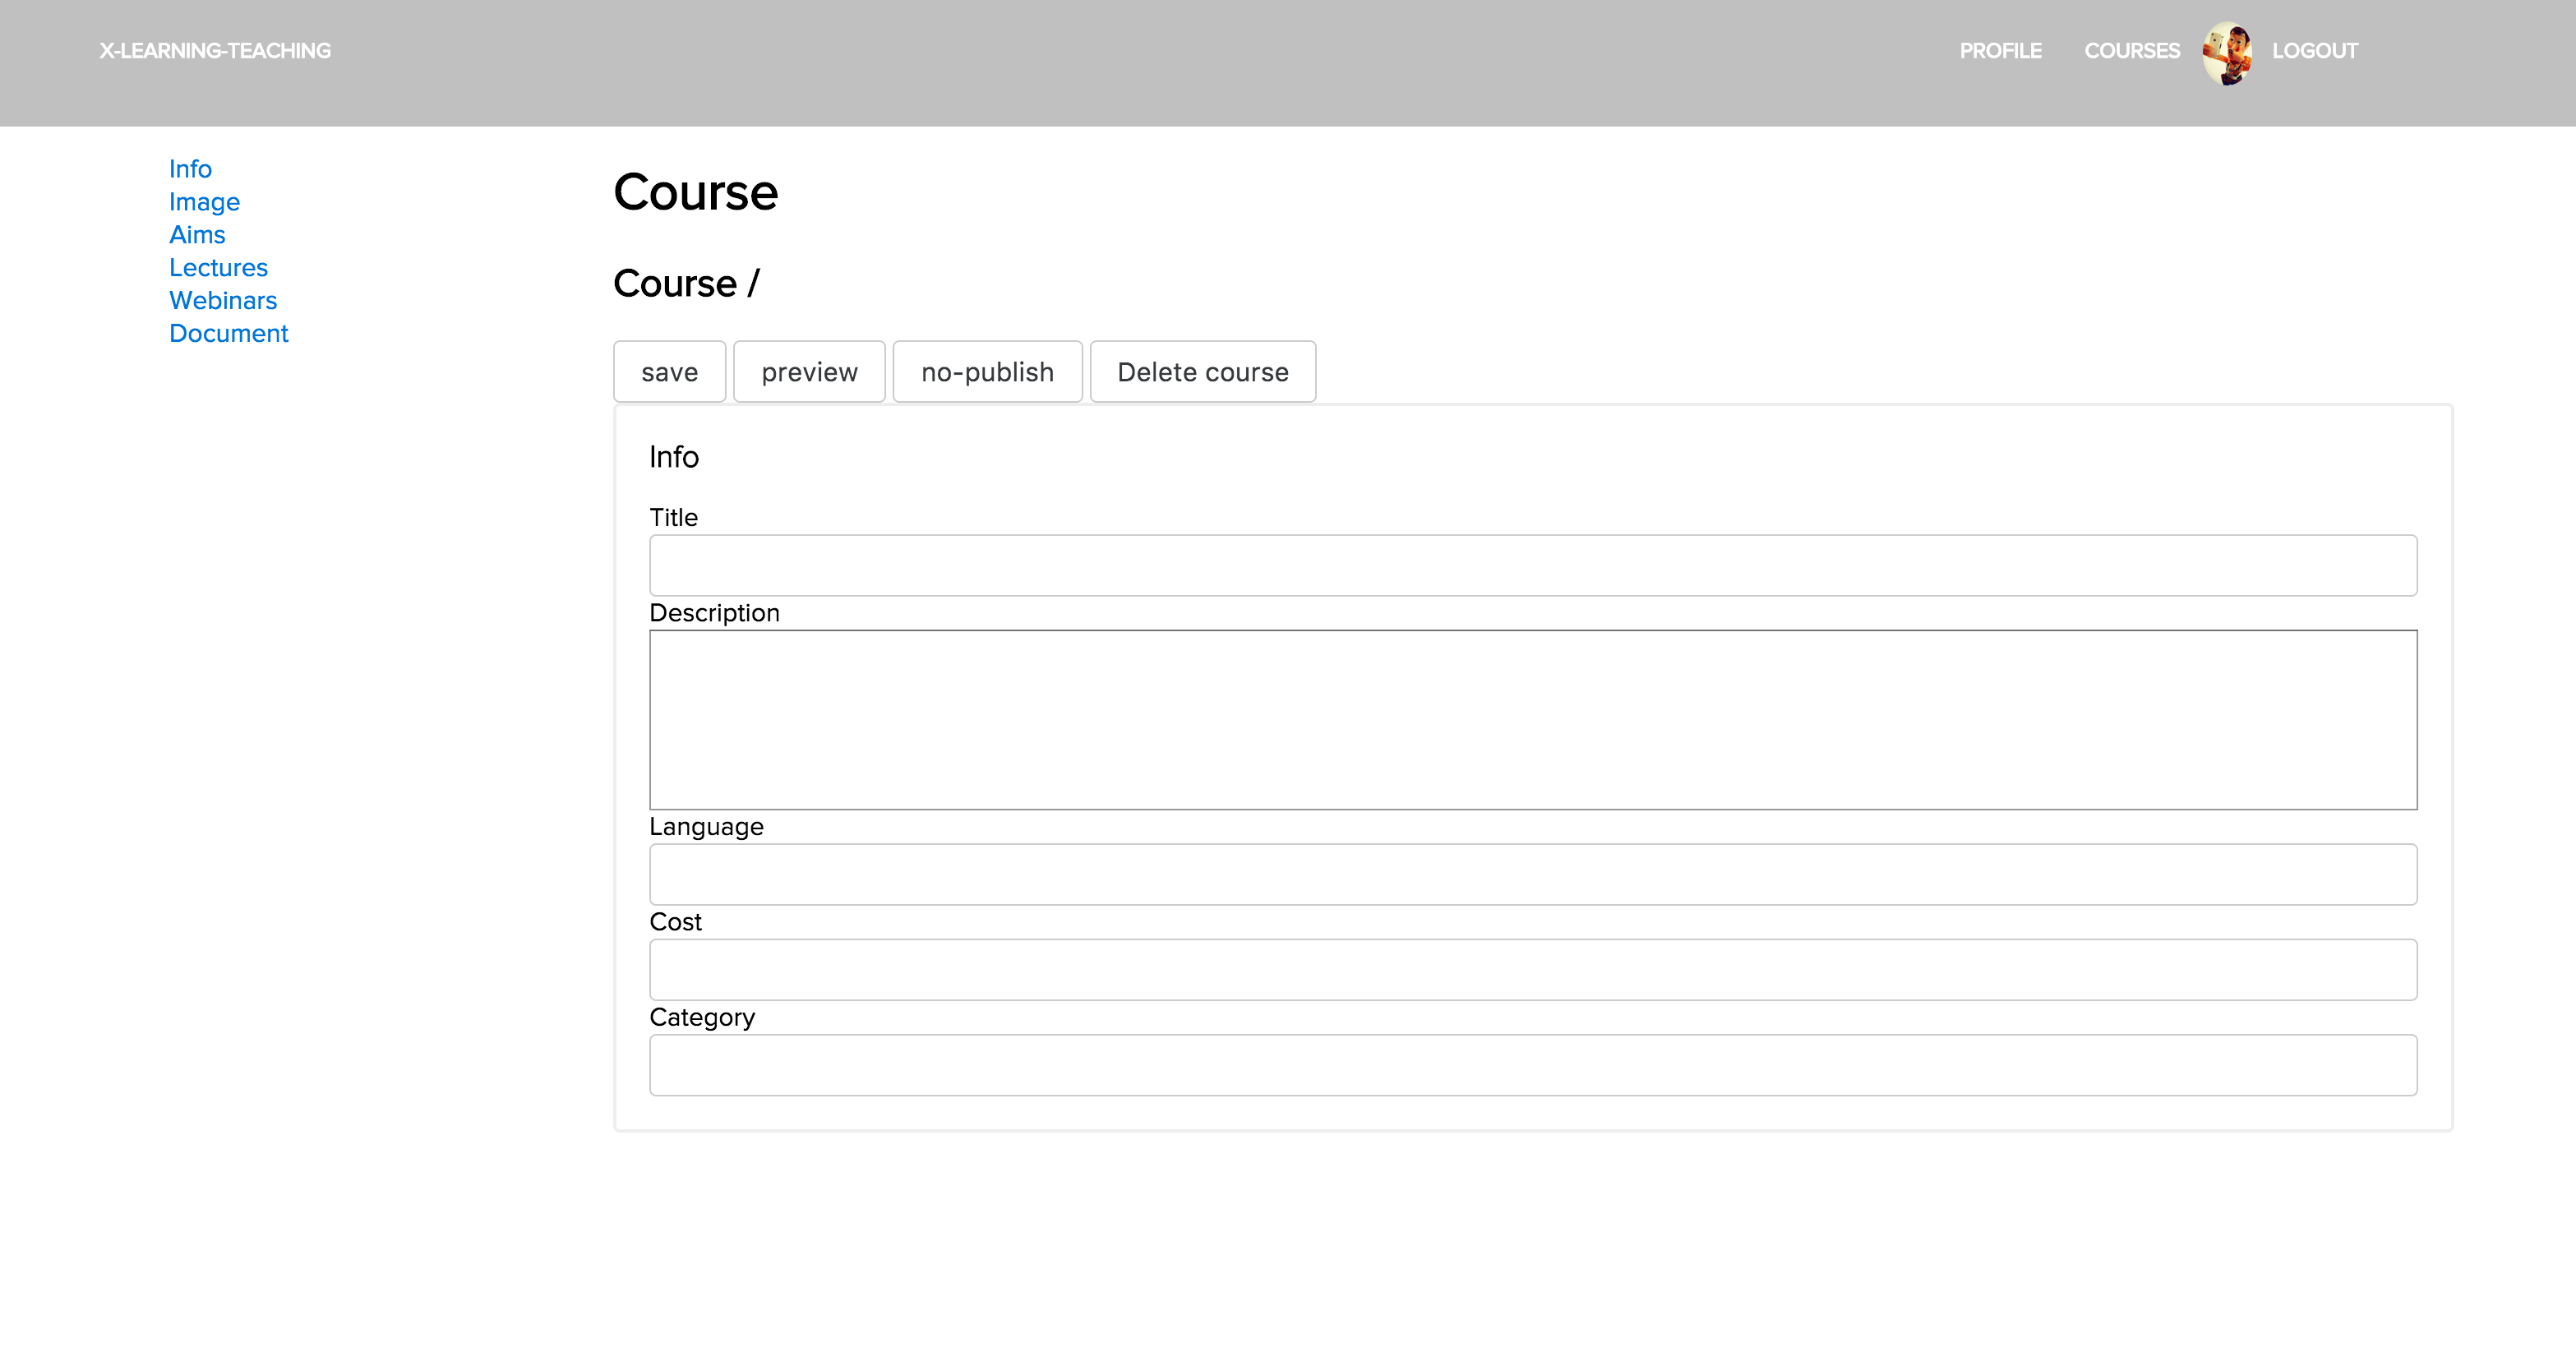
\includegraphics[width=1.0\linewidth]{images/chapter3/admin-course.png}\hfill
 \caption[Page Admin course]{Page Admin course}
 \label{fig:fourV}
\end{figure}


